\section{Motivation}

Supersonic Isothermal Turbulence is ubiquitous in astrophysical flows.  The low
density of gas in the interstellar medium allows for it to cool very
effectively, so the temperature stays roughly constant. Explosions of supernovae
drive flows with velocities more than 10 times the speed of sound in the ISM.
An important aspect of this is the high degree of compressibility of isothermal
gas.  Supersonic isothermal flows can make very large density contrasts, which
is essential for processes like the formation of stars.  We have developed
analytic models of the correlation of density, $\rho$, and velocity, $v$, that
will be useful in theoretical treatments of the interstellar medium.  We now
hope to verify these analytic models with high resolution simulations.  

The simulations to be performed will have periodic boundary conditions and begin
with a uniform density.  Turbulence is generated by adding a fixed driving
pattern to the velocity
 at large scale, and the chaos of the fluid
dynamics distributes that energy to all scales.  

We have developed analytic models for several quantities in such flows.  The
probability distribution function for both density and velocity are
traditionally modeled as a lognormal and Maxwellian, respectively, but our first
paper has shown that lognormal density is not accurate.  The next thing we are
verifying is the joint PDF of density and velocity, $f_{\rho,v}(\rho,v)$.  If
density and velocity are uncorrelated, which is often assumed, the joint PDF can be written as the
product of marginalized PDFs, $f_{\rho,v}(\rho,v)=f_\rho(\rho) f_v(v)$.  Our
preliminary low resolution simulations show that this is not true, and we have
developed a correction function, $g(\rho,v)$ such that 
$$
f_{\rho,v}(\rho,v)=f_\rho(\rho) f_v(v) + g(\rho,v).
$$

Supersonic isothermal turbulence can be parametrized by two free parameters: the
Mach number $\mach$, which is the
ratio of velocity to the local sound speed; and the forcing parameter, $\xi$,
which determines the amount of compressive motions in the driving velocity
pattern.
$\xi$ ranges between 0 and 1, with \xis\ representing only rotational motions,
and \xic\ denoting only compressive motions.  Typical mach numbers in the
interstellar medium range from 1
to about 10, though much faster flows do occur.  Our previous proposal fixed
$\xi=0.5$.  Now it is time to run $\xi=0,1$ to verify that the models are fully
general.  More compressibility in the driving pattern alters the density statistics and
thus the correlations.  Our low resolution study shows that our model is
accurate for all values of $\mach,\xi$ that were appropriate for that
resolution.

We will verify our models using a suite of twelve $1024^3$ simulations.  We will use
$\mach$ = (1,2,4,10), with forcing parameters $\xi=0,0.5,1$.  The $\mach=8$
simulations were performed in the fall, with $\xi=0,0.25,0.5,0.75,1$.  We will
only use three values of $\xi$ for the full suite, which brackets the range of
possible parameters.  This range of Mach numbers is important as the flow
properties change from weakly supersonic \mach=1 to highly supersonic \mach=10.
Higher values of \mach\ are of interest, but less common so will be omitted at
this time.

A resolution of $1024^3$ is necessary to properly reproduce the density
statistics.  Low resolution simulations have large zones, whence it is difficult
to get large densities, which in turn impacts the mean and variance measured
for a given Mach number.  This can be seen in Figure \ref{fig.sigma}, which
shows the standard deviation in density, $\sigma_\rho$, vs. the Mach number for
a suite of low resolution runs (black points) and our recently run $1024^3$ (red
point).  It
is theoretically expected that the two are linearly related, $\sigma_\rho = b
\mach$, but as can be seen from the Figure, the low resolution runs fall short.
The high resolution run is more in line with the linear relation.  Even higher 
resolution than $1024^3$ would be useful and interesting, but as the cost scales like the
fourth power of size, we cannot justify such an expense at this time.

Simulations will be run for 10\tdyn, where the dynamical time \tdyn=$0.5/\mach$.
This is the time for the driving flow to cross the box, which has a pattern size
of one half of the box.  This integration time is important to reduce the noise
in the joint distributions.  This can be seen in Figure \ref{fig.joint}, which
shows the joint $\rho-v$ distribution, $f_{\rho,v}(\rho,v)$.  First observe the right panel.  If the
two were uncorrelated, the distribution would be symmetric, instead of skewed.
Our analytic formula reproduces these contours.  The effect of time integration
can be seen by comparing the left and right panels.  The left panel was averaged
over 50 \tdyn, while the right was averaged over 100 \tdyn, substantially
increasing the signal-to-noise.  The high resolution runs, having more data
points, achieve convergence about an order of magnitude faster, so we will only
run the high resolution runs for 10\tdyn.  Since the noise decreases roughly
like shot noise, $1/\sqrt{t}$, further integration improves the noise slowly.


\begin{figure} \begin{center}
\caption[ ]{}
\label{fig.sigma} \end{center} \end{figure}

\begin{figure} \begin{center}
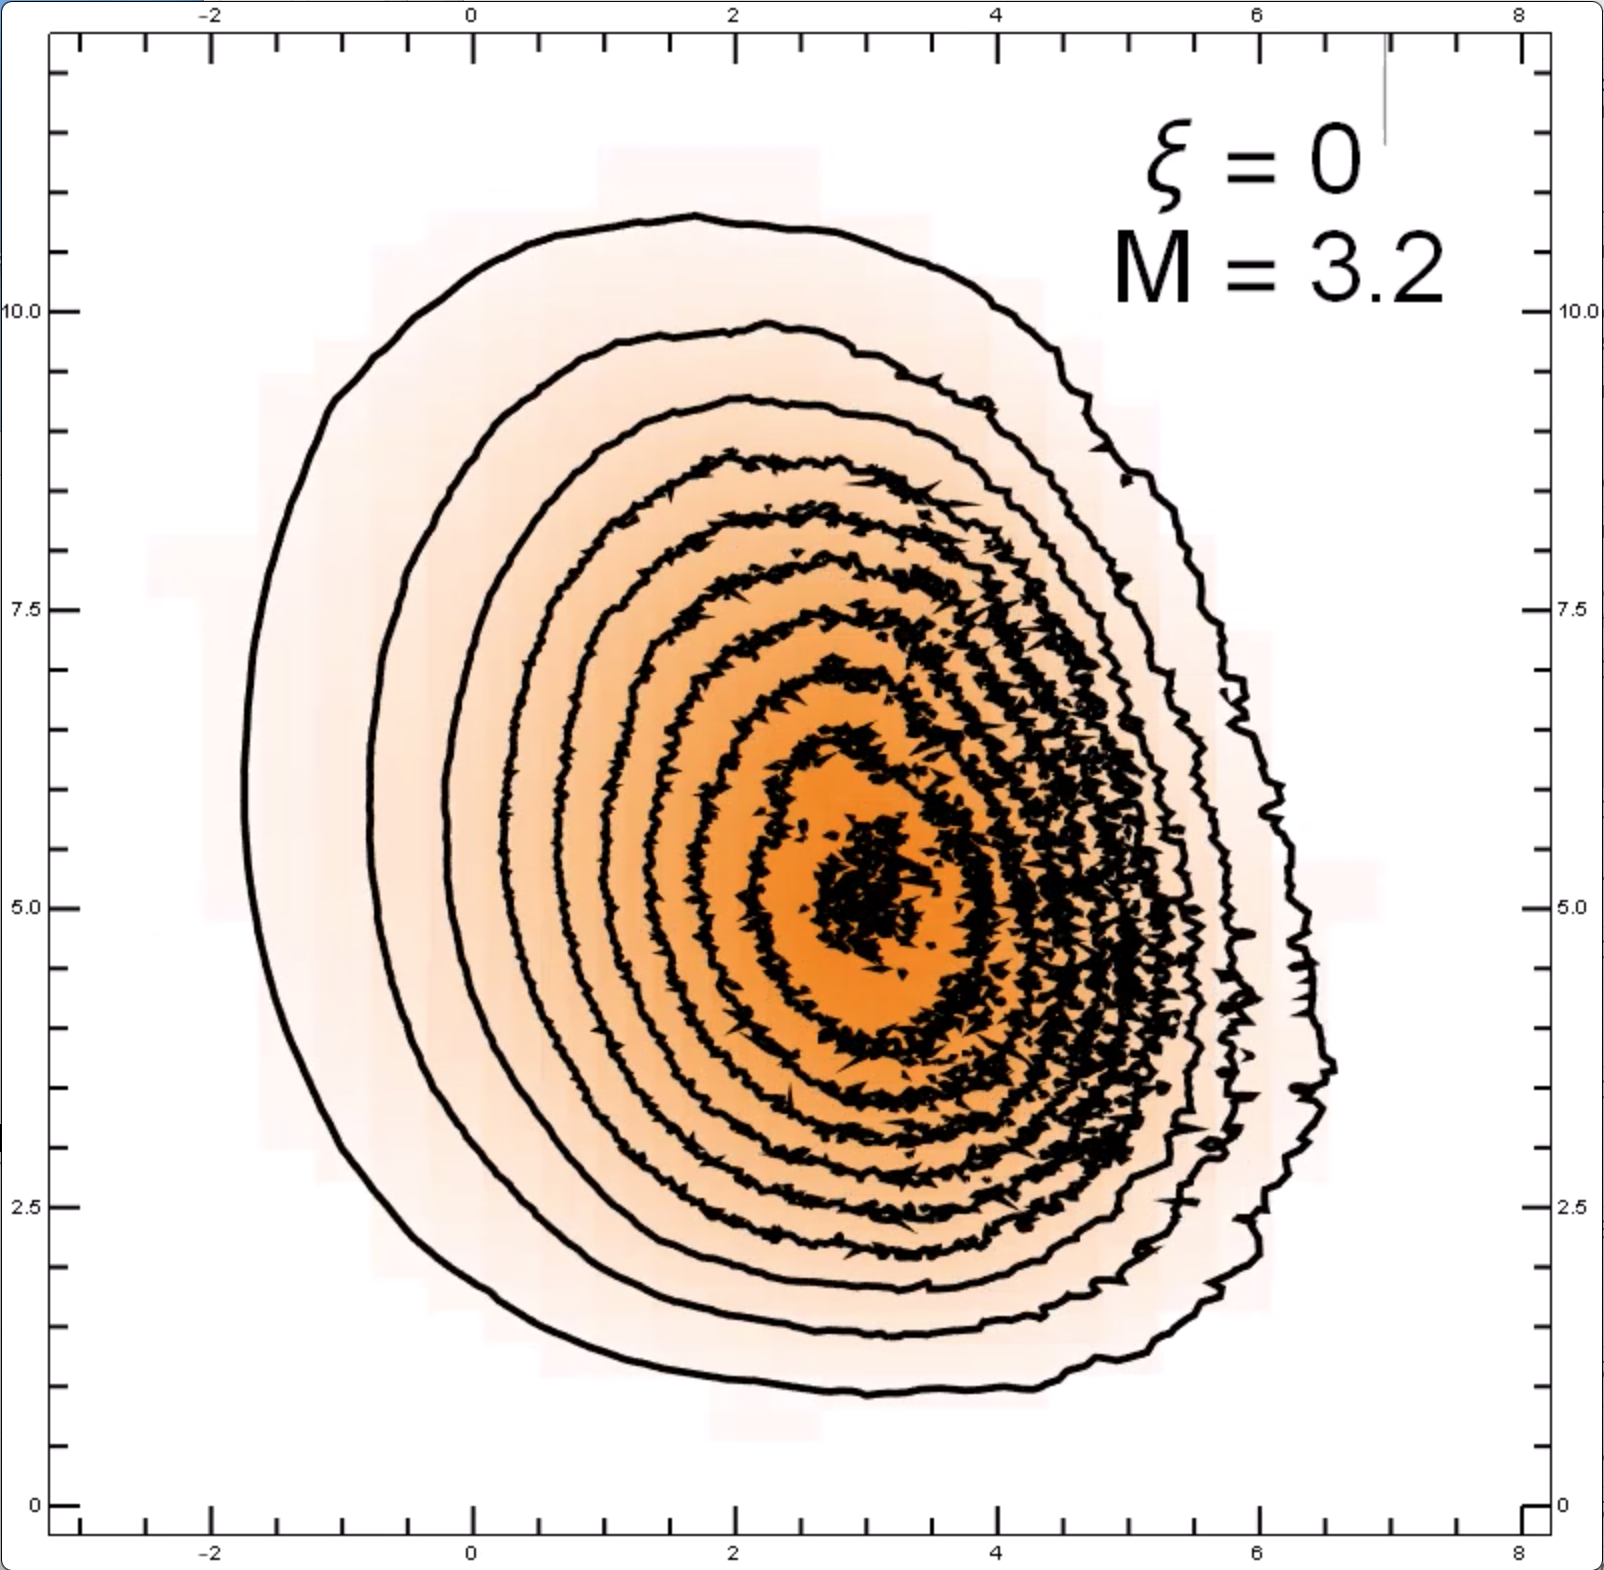
\includegraphics[width=0.27\textwidth]{Joint1.png}
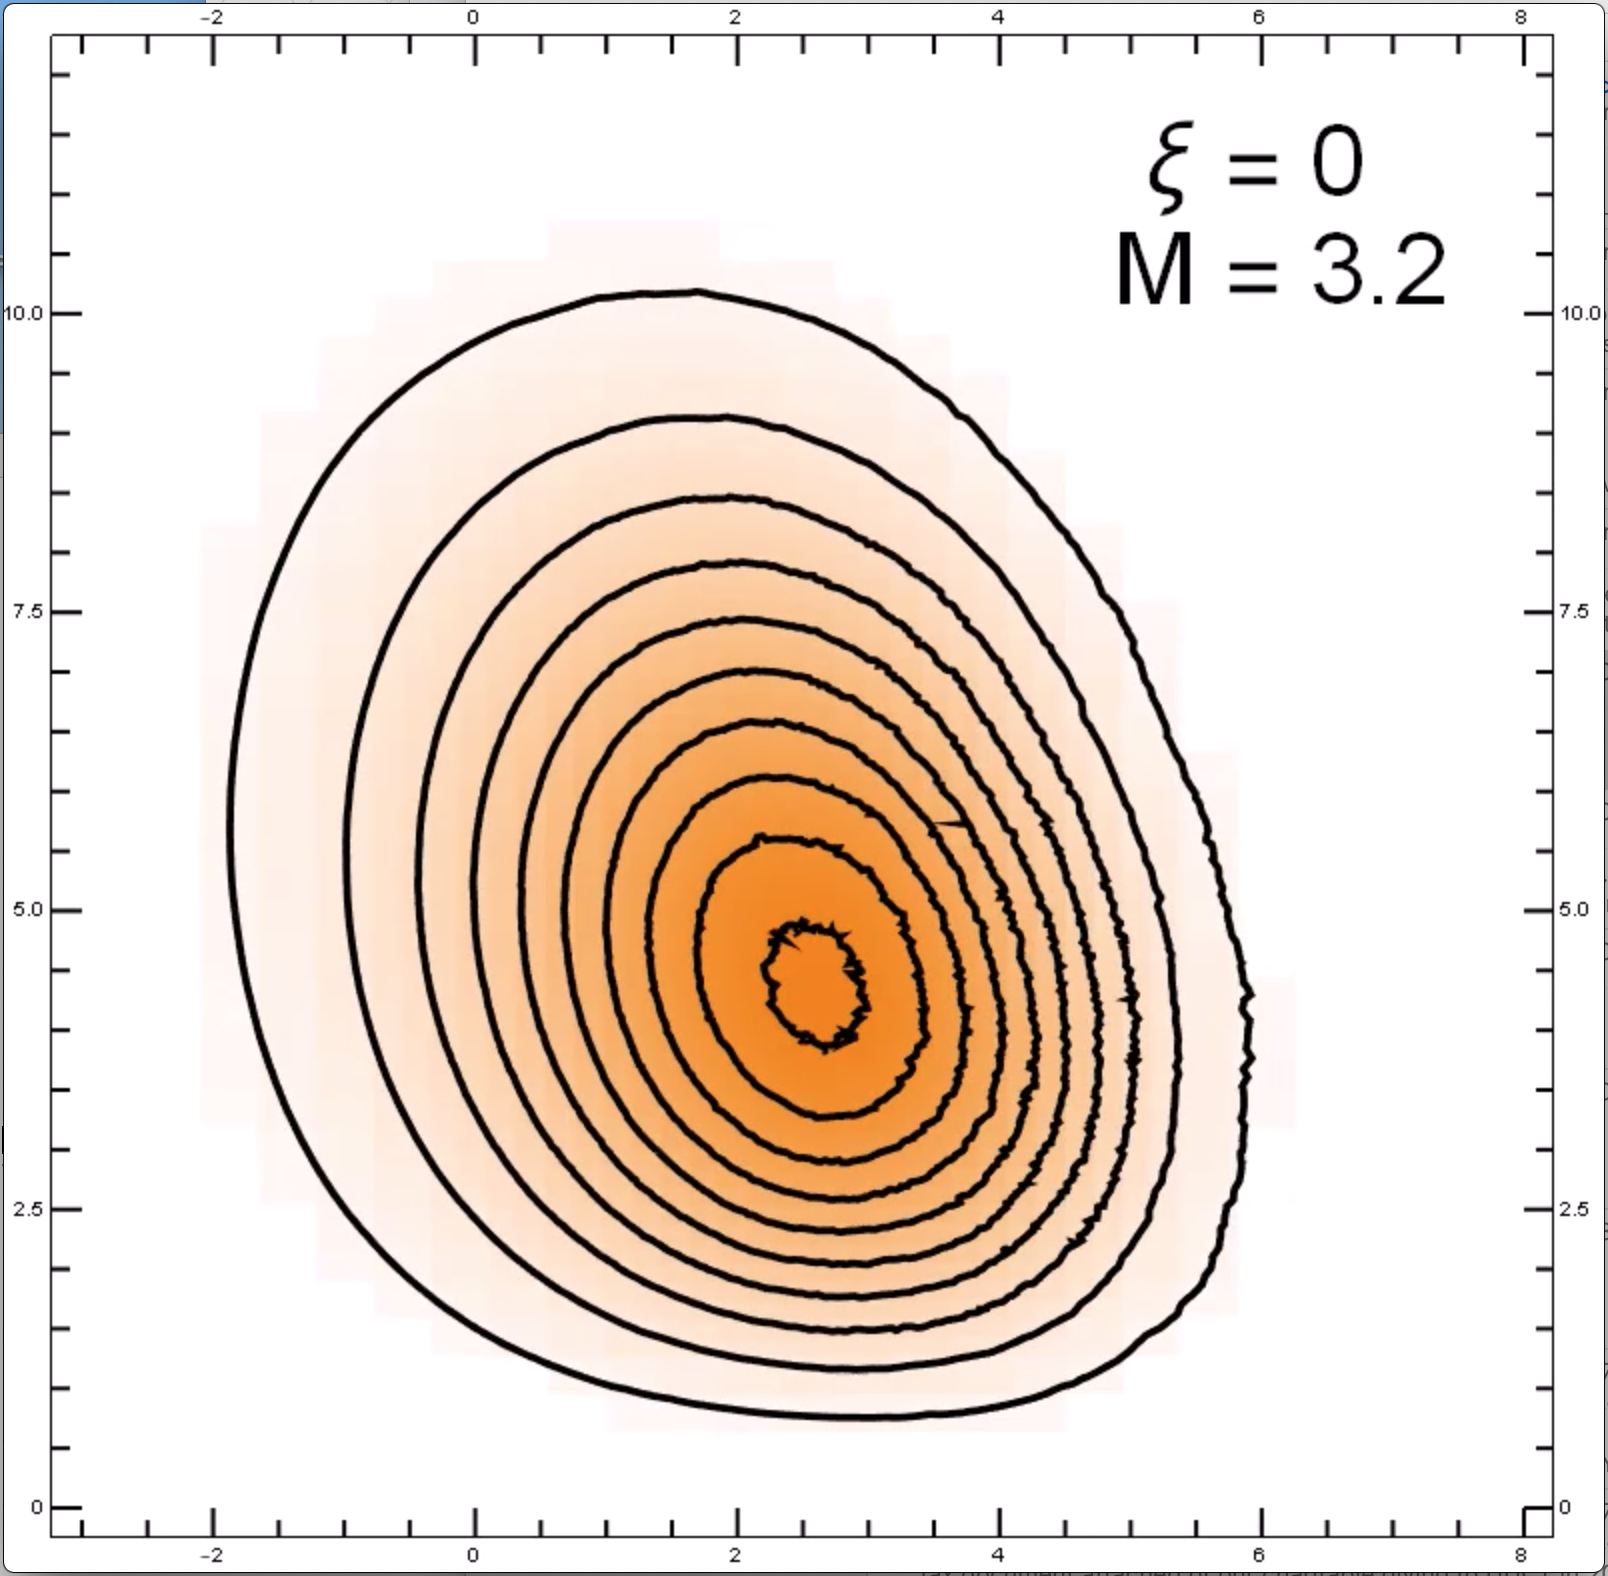
\includegraphics[width=0.27\textwidth]{Joint2.png}
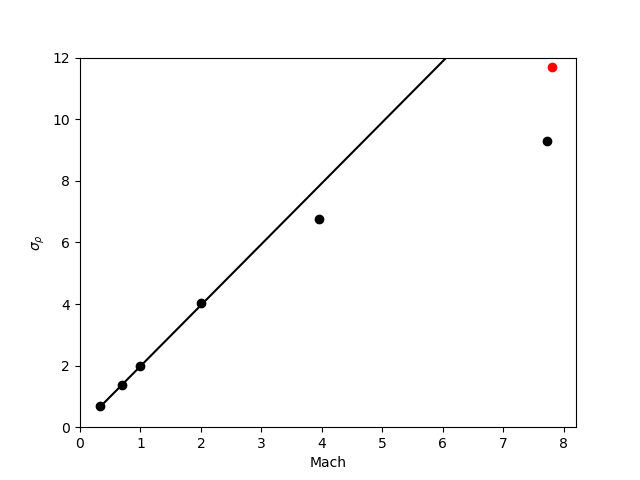
\includegraphics[width=0.40\textwidth]{resolution.png}
\caption[ ]{\emph{(Left, Center)} The joint distribution between density (horizontal) and velocity (vertical) for low resolution preliminary runs.  For uncorrelated variables, the joint distribution would be symmetric, while here we have a pronounced tilt.  The left panel shows an averaging window of 30\tdyn, while the right has averaged over 100 \tdyn. Higher resolution can be run for only 10\tdyn and achieve the same noise.
\emph{(Right)}
The relation between  the Mach number and the
variance in density, $\sigma_\rho$.  Black points show low resolution runs at
$256^3$, while the red point was run with $1024^3$ zones.  The low resolution
runs fail to reproduce the expected linear trend at large Mach numbers.  
}
\label{fig.joint} \end{center} \end{figure}
